\documentclass[a4paper,titlepage,dvipdfmx]{jarticle}
\usepackage{caption}
% 数式用
\usepackage{longtable}
\usepackage{amsmath, amsfonts}  % 数式用
\usepackage{bm} % 数式中の太字
\usepackage{amssymb} % 記号
% 画像用
\usepackage{float} % 画像の挿入箇所を固定
\usepackage[dvipdfmx]{graphicx} % 画像挿入用
\usepackage{wrapfig} % 画像の周りに本文を流し込み
% ページレイアウト
\usepackage{here} % 画像を強制的に出力
\usepackage{url} % URLリンク
\usepackage{hyperref} % 
\hypersetup{
  colorlinks=false, % リンクに色をつけない設定
  bookmarks=true, % 以下ブックマークに関する設定
  bookmarksnumbered=true, % ブックマークに節番号などをつけるか
  pdfborder={0 0 0}, % 枠なし
  bookmarkstype=toc % 目次情報のブックマークを作る
}
\usepackage{multirow} % 表で行結合
\usepackage[margin=20truemm]{geometry} %余白調整
% 文字装飾
\usepackage{color} % 文字色
\usepackage[table,xcdraw]{xcolor} % 表の色
\usepackage{ascmac} % 丸枠
\usepackage{fancybox} % 丸枠
\usepackage{booktabs} % 表の横線を調整するためのパッケージ
\usepackage{tabularx} % 表の幅を調整するためのパッケージ
\usepackage{tcolorbox} %ボックスやフレームを作成するためのパッケージ
% プログラム用
\definecolor{comment}{rgb}{0.52,0.60,0.00} %green
\usepackage{listings,jvlisting} %日本語のコメントアウトをする場合jvlisting(もしくはjlisting)が必要
%ここからソースコードの表示に関する設定
\lstset{
  basicstyle=\ttfamily,
  showstringspaces=false,
  commentstyle=\color{comment},
  keywordstyle= \color{blue}\bfseries,
  xleftmargin=0zw, %左余白
  xrightmargin=0zw,%右余白
  frame=single,%枠線
  frameround=tttt,%枠線角丸
}
\usepackage{fancyhdr} % ヘッダー・フッター
\pagestyle{fancy}
    % \lhead{専門チャレンジ(PCプログラミング)} %ヘッダ左
    \chead{第1回 Pythonに触れてみよう} %ヘッダ中央
    \rhead{授業資料} %ヘッダ右
    \cfoot{\thepage} %フッタ中央.ページ番号を表示
    \rfoot{\today} %フッタ右
    \renewcommand{\headrulewidth}{0.4pt} %ヘッダの線の太さ
    \renewcommand{\footrulewidth}{0.4pt} %フッタの線の太さ
    
\begin{document}
\section{はじめに}
Pythonは、オブジェクト指向スクリプト言語の一つであり、
プログラミング初学者にとって難しく感じる、「型」や「メモリ管理」を意識せずにプログラムを書くことができる言語です。
また、Pythonは有志の人々によってさまざまなライブラリ\footnote{プログラムにおいてよく利用される機能を切り出して、再利用しやすいようにまとめたもの}が
開発されており、それらを利用することで、短いコードで多くのことを実現することができます。

近年ではAIなどの発展によってさらに注目されるようになっており、
学習する価値の高い言語と言えるでしょう。
\section{環境構築}
Pythonを使うためには、Pythonのインストールが必要です。
今回は簡単のために直接Pythonのインストールを行います。
\subsection{Pythonのインストール}
\url{https://www.python.org/downloads/}にアクセスし、Pythonのインストーラをダウンロードします。
今回の授業では最も最新のPython3.12.3をダウンロードします。
\begin{figure}[H]
  \centering
  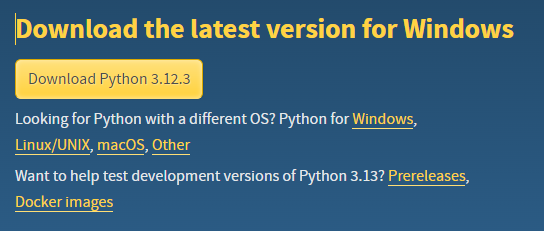
\includegraphics[width=10cm]{./figs/python-download.png}
  \caption{Pythonのダウンロード}
\end{figure}

ダウンロードしたインストーラを実行し、Pythonをインストールします。
\begin{figure}[H]
  \centering
  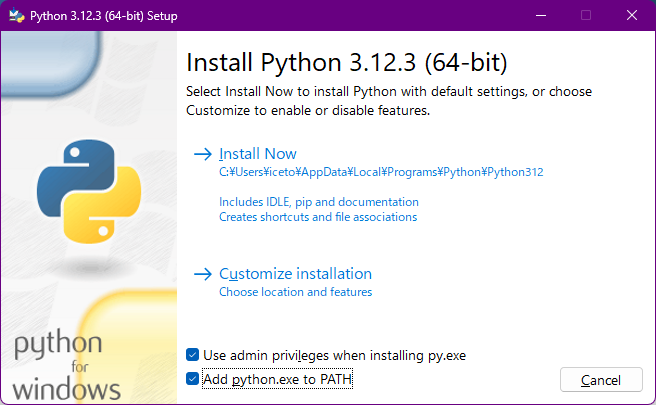
\includegraphics[width=10cm]{./figs/python-install.png}
  \caption{Pythonのインストール}
\end{figure}
``Add python.exe to PATH''にチェックをいれて、``Install Now''をクリックします。
これで、Pythonのインストールは完了です。

\subsection{エディタのインストール}
Pythonのプログラムを書くためには、エディタが必要です。
OS内臓のテキストエディタでも記述することはできますが、
プログラムの書きやすさを考えると、専用のエディタを使うことをおすすめします。
今回用いるエディタは、Visual Studio Codeです。
\url{https://code.visualstudio.com/}にアクセスし、Visual Studio Codeをダウンロードします。

\begin{figure}[H]
  \centering
  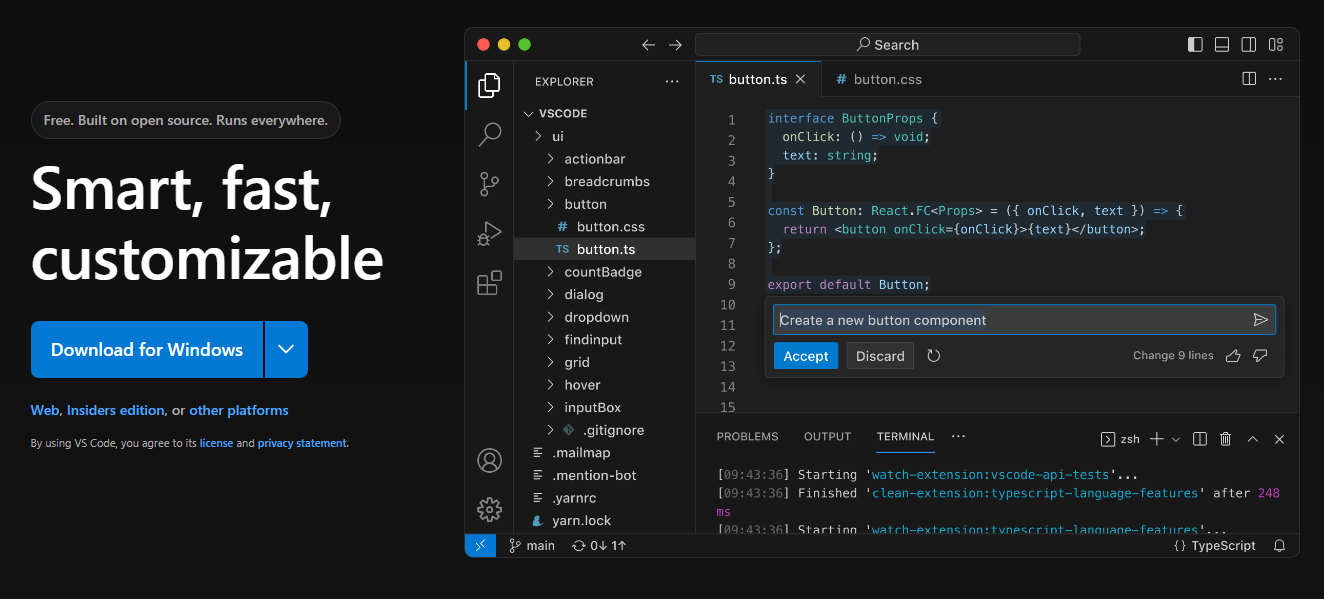
\includegraphics[width=10cm]{./figs/vscode-download.png}
  \caption{Visual Studio Codeのダウンロード}
\end{figure}

\begin{figure}[H]
  \centering
  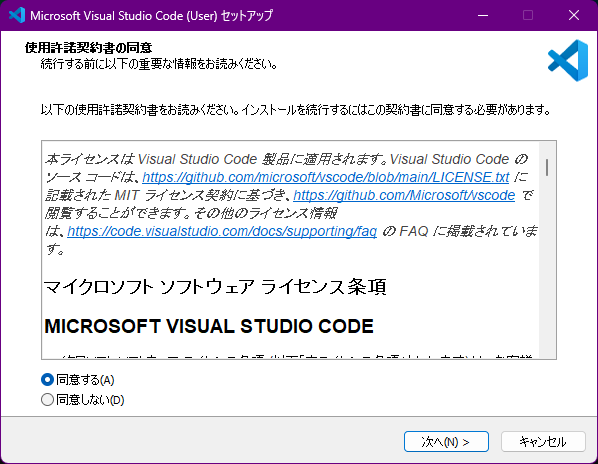
\includegraphics[width=10cm]{./figs/vscode-install1.png}
  \caption{Visual Studio Codeのインストール1}
\end{figure}
使用許諾に同意をして、``次へ''をクリックします。

\begin{figure}[H]
  \centering
  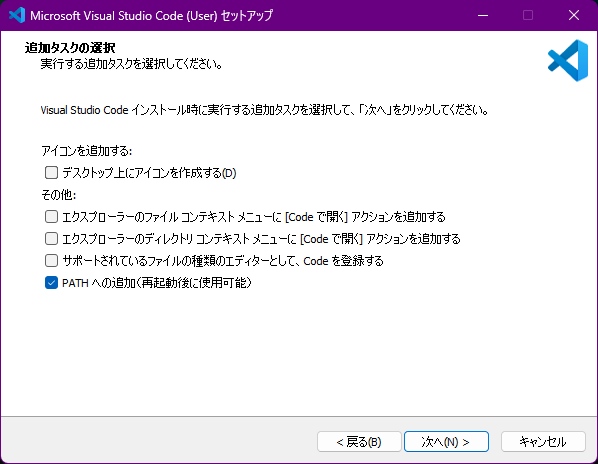
\includegraphics[width=10cm]{./figs/vscode-install2.png}
  \caption{Visual Studio Codeのインストール2}
\end{figure}
``追加のタスクの選択''で、``パスに追加''にチェックを入れて、``次へ''をクリックします。

\begin{figure}[H]
  \centering
  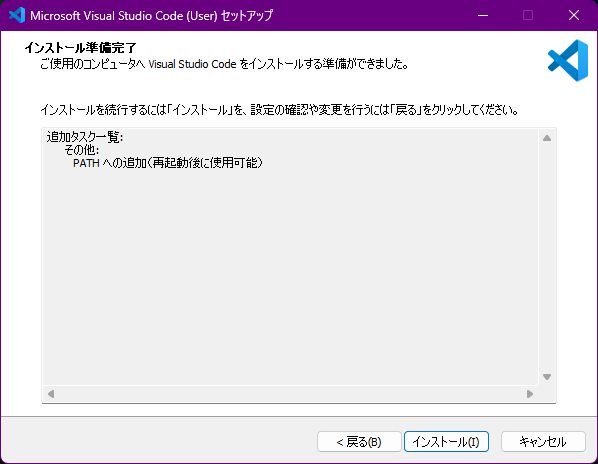
\includegraphics[width=10cm]{./figs/vscode-install3.png}
  \caption{Visual Studio Codeのインストール3}
\end{figure}
``インストール''をクリックします。

以上で、Visual Studio Codeのインストールは完了です。

\section{Pythonの基本}
\subsection{Hello World\protect\footnote{Hello Worldはプログラミング初学者が最初に書く慣例的なプログラムです。}}
Pythonのプログラムは、拡張子が``.py''のファイルに記述します。
まずは、Hello Worldを表示するプログラムを書いてみましょう。
Visual Studio Codeを起動し、新しいファイルを作成します。
ファイル名を``hello.py''とし、以下のプログラムを記述します。
\begin{lstlisting}[caption=hello.py]
print("Hello World")
\end{lstlisting}
プログラムを実行するには、ターミナルを開き、以下のコマンドを実行します。
\begin{lstlisting}
python hello.py
\end{lstlisting}
``Hello World''と表示されれば、プログラムの実行は成功です。


\end{document}